\documentclass{article}
\usepackage[top=3cm, bottom=3cm, left=3.5cm, right=3.5cm]{geometry}
\usepackage{amsmath}
\usepackage[portuguese]{babel}
\usepackage{listings}
\usepackage{xcolor}
\usepackage[utf8]{inputenc}
\usepackage{graphicx}
\usepackage{csquotes}
\usepackage{url}
\usepackage{hyperref} % Add this package for hyperlinks
\usepackage{indentfirst}
\usepackage{float}


\definecolor{backcolour}{rgb}{0.95,0.95,0.92}

\lstdefinestyle{mystyle}{
    backgroundcolor=\color{backcolour},   
    basicstyle=\ttfamily\footnotesize,
    breakatwhitespace=false,         
    breaklines=true,                 
    captionpos=b,                    
    keepspaces=true,                 
    numbers=left,                    
    numbersep=5pt,                  
    showspaces=false,                
    showstringspaces=false,
    showtabs=false,                  
    tabsize=2
}

\lstset{style=mystyle}

\title{\textbf{SME0206 -- Fundamentos de An\'{a}lise Num\'{e}rica - Trabalho Pr\'{a}tico \#1}}
\author{Gabriel Coutinho Chaves \\ 15111760 \and Theo Urbano Gaudencio de Sene \\ 12558717 \and Ian De Holanda \\ 13835412}
\date{\today}

\begin{document}


\maketitle

% -----------------------------------------------------------------------------

\section{Introdu\c{c}\~{a}o}
Este relatorio aborda o tema de m\'{e}todos num\'{e}ricos para encontrar ra\'{i}zes de fun\c{c}\~{o}es, com foco espec\'{i}fico na fun\c{c}\~{a}o polinomial do quinto grau


\begin{equation}
    f(x) = 63x^5 - 381x^4 + 496x^3 + 204x^2 - 544x + 192
\label{eq:1}
\vspace*{4pt}
\end{equation}
nos intervalos [0,1] e [1,2].


O objetivo principal \'{e} analisar e comparar diferentes m\'{e}todos num\'{e}ricos para encontrar as ra\'{i}zes desta fun\c{c}\~{a}o, incluindo:

\begin{itemize}
    \item M\'{e}todo da Bisse\c{c}\~{a}o
    \item M\'{e}todo de Newton
    \item M\'{e}todo das Secantes
\end{itemize}

Utilizamos a linguagem de programa\c{c}\~{a}o Python \cite{python}, por meio da interface de desenvolvimento Jupyter Lab \cite{jupyter}, para implementar e testar estes m\'{e}todos, buscando compreender suas caracter\'{i}sticas, efici\^{e}ncia e precis\~{a}o na resolu\c{c}\~{a}o do problema proposto.


% -----------------------------------------------------------------------------


\section{M\'{e}todos e Procedimentos}
Nesta se\c{c}\~{a}o, apresentaremos os m\'{e}todos num\'{e}ricos implementados para encontrar as ra\'{i}zes da fun\c{c}\~{a}o \eqref{eq:1}. Descreveu-se os c\'{o}digos em Python, detalhando as principais subrotinas, suas vari\'{a}veis de entrada e sa\'{i}da, bem como as decis\~{o}es de implementa\c{c}\~{a}o e dificuldades encontradas.

Para todos os métodos implementados, usamos um critério de parada baseado na tolerância e no número máximo de iterações, garantindo que os algoritmos forneçam uma aproximação adequada da raiz em tempo razoável. Fixamos o número máximo de iterações em 50 e utilizamos o erro $\epsilon=10^{-6}$.

\subsection{Defini\c{c}\~{a}o da Fun\c{c}\~{a}o e da sua Primeira Derivada}

Para todos os m\'{e}todos implementados, estabeleceu-se a seguinte fun\c{c}\~{a}o polinomial e sua derivada, definidas como express\~{o}es lambda em Python:

\begin{lstlisting}[language=Python]
f = lambda x: 63*x**5 - 381*x**4 + 496*x**3 + 204*x**2 - 544*x + 192
dfdx = lambda x: 315*x**4 - 1524*x**3 + 1488*x**2 + 408*x - 544
\end{lstlisting}

Onde:
\begin{itemize}
    \item \texttt{f(x)} representa a fun\c{c}\~{a}o polinomial \eqref{eq:1};
    \item \texttt{dfdx(x)} representa a sua primeira derivada.
\end{itemize}

Estas defini\c{c}\~{o}es s\~{a}o utilizadas como par\^{a}metros de entrada nos m\'{e}todos que requerem a fun\c{c}\~{a}o e/ou sua derivada, como o m\'{e}todo de Newton e o m\'{e}todo das Secantes.

\subsection{An\'{a}lise dos Intervalos e Ra\'{i}zes}

Para visualizar as ra\'{i}zes e os intervalos de interesse, geramos dois gr\'{a}ficos utilizando a biblioteca Matplotlib \cite{matplotlib}, um para cada intervalo.

\begin{figure}[h]
\centering
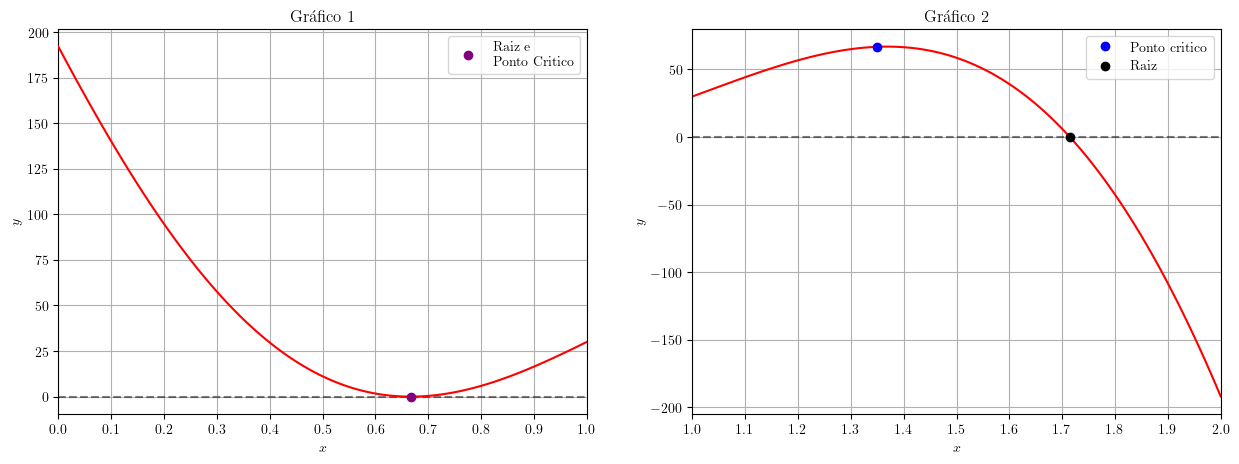
\includegraphics[width=\textwidth, keepaspectratio]{output.png}
\caption{Gr\'{a}fico da fun\c{c}\~{a}o f(x) nos intervalo $[0,1]$ e $[1,2]$}
\label{fig:funcao_grafico}
\end{figure}

Observando o Gr\'{a}fico 1 da Figura \ref{fig:funcao_grafico}, suspeita-se da existência de uma raiz entre $0,6$ e $0,7$. Ademais, graficamente pode-se conjecturar que este mesmo ponto pode também ser um ponto de mínimo local.

Já no Gráfico 2 da Figura \ref{fig:funcao_grafico}, é certa a existência de raiz pelo Teorema do Valor Intermediário, uma vez que existem valores positivos e negativos para a função. Graficamente, esse valor é próximo de $1,7$. Além disso, pode-se evidenciar a existência de um ponto de crítico entre $1,3$ e $1,4$.
\\


Para analisar de maneira mais exata as ra\'{i}zes da fun\c{c}\~{a}o, utilizamos a biblioteca SymPy \cite{sympy} para operações com matemática simbólica.

Definiu-se uma variável simbólica \textbf{x} e a expressão \textbf{h} desta variável de acordo com a função \eqref{eq:1}. Então, utilizou-se do método \textit{\textbf{smp.solve}}, que encontra as raízes da expressão fornecida.
  
\begin{lstlisting}[language=Python]
x = smp.symbols('x') 
h =  63*x**5 - 381*x**4 + 496*x**3 + 204*x**2 - 544*x + 192
sol = smp.solve(h,x,numerical=True )
\end{lstlisting}




Assim, obteve-se a lista \textbf{\textit{sol}} de soluções (raízes) da função em questão, que é a seguinte:

\begin{equation}
[-1, \frac{2}{3}, \frac{12}{7}, 4]
\label{eq:sol}
\end{equation}

Em particular, interessar-nos-ão as soluções $\frac{2}{3}$ e $\frac{12}{7}$, que são as únicas que estão nos intervalos que serão abordados neste relatório. E cujo valor decimal aproximado foi obtido utilizando o método \textbf{smp.evalf} da biblioteca SymPy.
\begin{lstlisting}[language=Python]
    sol[1].evalf()
\end{lstlisting}
Resultado:
0.666666666666667
\begin{lstlisting}[language=Python]
    sol[2].evalf()
\end{lstlisting}
Resultado:
1.71428571428571\\

Como a função \eqref{eq:1} é uma função do quinto grau, pelo Teorema Fundamental da Álgebra, ela deve ter 5 raízes complexas (incluindo a possível multiplicidade delas) \cite{wikipedia}. Como pode-se obervar, o método \textbf{\textit{smp.solve}} retornou apenas 4 raízes, portanto deve-se suspeitar que alguma delas têm multiplicidade 2. 

Com efeito, se realizarmos uma divisão de polinômios da expressão definida em \textbf{h} por $(x-\frac{2}{3})$ o polinômio obtido tem a mesma lista de soluções de \eqref{eq:sol}, consequentemente, $\frac{2}{3}$ ainda é solução, logo $x=\frac{2}{3}$ é uma raiz múltipla. Esse fato é relevante pois interfere na velocidade de convergência de algum dos métodos que foram utilizados.


% -----------------------------------------------------------------------------


\subsection{M\'{e}todo da Bisse\c{c}\~{a}o}
O Método da Bisseção é um tipo de método de quebra, uma classe de métodos para aproximação de raízes que funciona "a partir de um intervalo
que contenha uma raiz da função e vai particionando este intervalo em outros menores, que ainda
contenham a raiz"  \cite{lobao}. 

O funcionamento deste algoritmo se fundamenta no Teorema do Valor Intermediário (TVI), que garante a existência de pelo menos uma raiz entre dois pontos em que a função continua tem valores com sinais distintos. 

Neste método são definidos um intervalo e uma função contínua nesse intervalo. Se os extremos avaliados na função tiverem produto negativo, isso significa que possuem sinais distintos. Nesse caso, há raiz no intervalo. Toma-se então a média aritmética dos extremos e checa-se com qual dos extremos o produto com a média obtida ainda é negativo. Esse processo pode ser repetido pra chegar numa aproximação tão boa quanto se deseje.
\\\\
Na implementação em Python foi feita da seguinte maneira:
\\

Vari\'{a}veis de entrada:
\begin{itemize}
    \item f: fun\c{c}\~{a}o para a qual estamos buscando a ra\'{i}z (ela precisa ser contínua)
    \item a, b: extremidades do intervalo inicial
    \item e: toler\^{a}ncia para o crit\'{e}rio de parada
    \item kmax: n\'{u}mero m\'{a}ximo de itera\c{c}\~{o}es permitidas
\end{itemize}

Vari\'{a}vel de sa\'{i}da:
\begin{itemize}
    \item x: aproxima\c{c}\~{a}o da ra\'{i}z encontrada
\end{itemize}

A rotina começa  definindo \textit{fa} e \textit{fb}, respectivamente a função avaliada em $a$ e $b$, e é conferido se já são são nulos, isto é, se um dos extremos é raiz. Caso seja, o programa encerra e devolve $a$ ou de $b$. Do contrário, checa-se se a função avaliada nos extremos têm sinal opostos, calculando o produto e avaliando se ele é negativo, ou seja, garantindo que há raiz no intervalo.

\begin{lstlisting}[language=Python]
    if fa == 0:
        return a
    elif fb == 0:
        return b
    elif fa * fb > 0:
        print('Erro. f(a) e f(b) tem o mesmo sinal.')
        return np.nan
\end{lstlisting}

Caso comprove-se a existência de raiz no intervalo $[a,b]$, $x_0$ é definida como $a$ e é calculada a média dos extremos e esse valor é chamado \textbf{x}. Encontra-se o valor da função em x e esse valor é comparado com \textit{fa} e \textit{fb} por meio do produto. Onde houver garantia de raiz, repete-se o processo.   

\begin{lstlisting}
    x = (a + b) / 2
    fx = f(x)
    erro = norm(x - x0)
        
    if fx == 0 or erro < e * (1 + norm(x)):
        return x
        
    if fx * fa < 0:
        b = x
    else:
        a, fa = x, fx
        
\end{lstlisting}
% -----------------------------------------------------------------------------


\subsection{M\'{e}todo de Newton}
O M\'{e}todo de Newton, tamb\'{e}m conhecido como m\'{e}todo de Newton-Raphson, \'{e} uma t\'{e}cnica iterativa que utiliza a primeira derivada da fun\c{c}\~{a}o para encontrar suas ra\'{i}zes. Este m\'{e}todo converge quadraticamente para ra\'{i}zes simples, o que o torna muito eficiente desde que não se tenha raízes múltiplas \cite{atk}. 

O Método de Newton fundamenta-se na expressão da primeira derivada da função. Como deseja-se encontrar a raiz $f(x)$ irá se anular, então teremos: 
$$f'(x_0)\approx\frac{f(x)-f(x_0)}{x-x_0} \Longleftrightarrow  x \approx x_0 - \frac{f(x_0)}{f'(x_0)}$$

Assim, utilizamos essa aproximação para obter a seguinte fórmula iterativa:

\begin{equation}
    x_{k+1} = x_k - \frac{f(x_k)}{f'(x_k)}
    \label{newton}
\end{equation}

Implementamos este m\'{e}todo da seguinte maneira:
\\

Vari\'{a}veis de entrada:
\begin{itemize}
    \item f: fun\c{c}\~{a}o para a qual estamos buscando a ra\'{i}z
    \item dfdx: derivada da fun\c{c}\~{a}o f
    \item x0:  o valor inicial para começar as iterações
    \item e: toler\^{a}ncia para o crit\'{e}rio de parada
    \item kmax: n\'{u}mero m\'{a}ximo de itera\c{c}\~{o}es permitidas
\end{itemize}

Vari\'{a}vel de sa\'{i}da:
\begin{itemize}
    \item x: aproxima\c{c}\~{a}o da ra\'{i}z encontrada
\end{itemize}

Nossa implementa\c{c}\~{a}o calcula \textbf{fx} e \textbf{dfdx} avaliadas no valor inicial \textbf{x0}. Em seguida inicia-se um \textit{loop} de no máximo \textbf{kmax} iterações em que a cada iteração é calculado

\begin{lstlisting}[language=Python]
    x = x0 - fx0/dfdx0
\end{lstlisting}
e checa-se se esse novo valor \textbf{x} obtido é próximo do valor \textbf{x0}. Caso a distância entre esses dois valores seja menor que o erro desejado $\epsilon$, então \textbf{x} está próximo da raiz exata da função de acordo com o erro estabelecido, por isso o programa encerra e retorna \textbf{x}.

Caso a distância entre \textbf{x} e \textbf{x0} seja maior que $\epsilon$, repete-se o processo declarando \textbf{x0} = \textbf{x}.

\begin{lstlisting}[language=Python]
    if norm(x-x0)<e*(1+norm(x)):
            return (x)
        x0 = x
        fx0 = f(x0)
        dfdx0 = dfdx(x0)
        k+=1
\end{lstlisting}



Uma poss\'{i}vel limita\c{c}\~{a}o deste m\'{e}todo \'{e} que ele pode falhar se a primeira derivada se aproximar de zero, o que pode ocorrer se a estimativa inicial estiver longe da ra\'{i}z ou se houver ra\'{i}zes m\'{u}ltiplas. Ademais, o m\'{e}todo requer o conhecimento expl\'{i}cito da derivada da fun\c{c}\~{a}o, além de que ela seja diferenciável, o que nem sempre \'{e} poss\'{i}vel ou pr\'{a}tico.

% -----------------------------------------------------------------------------

\subsection{M\'{e}todo das Secantes}
O m\'{e}todo das secantes \'{e} uma varia\c{c}\~{a}o do m\'{e}todo de Newton que n\~{a}o requer o c\'{a}lculo expl\'{i}cito da derivada, utilizando o Polinômio de Taylor do Primeiro Grau como aproximação para a ela. 

O Polinômio de Taylor do Primeiro Grau num ponto é dado pela expressão: 

$$P(x) = f(x_0) + f'(x_0)(x-x_0)$$
portanto pode-se substituir a primeira derivada em \eqref{newton} obtendo assim:

\begin{equation}
    x_{k+1} = x_k - \frac{f(x_k)(x_{k}-x_{k-1})}{f(x_k)-f(x_{k-1})}
\end{equation}
uma vez que $P(x)=0$, já que queremos encontra uma aproximação para a raiz.\\

Implementamos este m\'{e}todo como segue:

Vari\'{a}veis de entrada:


\begin{itemize}
    \item f: fun\c{c}\~{a}o para a qual estamos buscando a ra\'{i}z
    \item x0, x1: duas estimativas iniciais pr\'{o}ximas \`{a} ra\'{i}z
    \item e: toler\^{a}ncia para o crit\'{e}rio de parada
    \item kmax: n\'{u}mero m\'{a}ximo de itera\c{c}\~{o}es permitidas
\end{itemize}

Vari\'{a}vel de sa\'{i}da:
\begin{itemize}
    \item x: aproxima\c{c}\~{a}o da ra\'{i}z encontrada
\end{itemize}

O código é similar ao Método de Newton, com a diferença que \textbf{x} é calculado por
\begin{lstlisting}[language=Python]
    x = x1 - fx1*(x1-x0)/(fx1-fx0)
\end{lstlisting}
e é feita uma troca de variáveis em que \textbf{x0} recebe o valor de \textbf{x1} e \textbf{x1} recebe o valor de \textbf{x}. No restante, o processo iterativo é análogo à implementação do Método de Newton.


Uma limitação deste método é a possibilidade de falha se a diferença entre f(x1) e f(x0) se aproximar de zero. No entanto, ele tem a vantagem de não requerer o cálculo explícito da derivada.
\begin{lstlisting}[language=Python]
    x0 = x1
    x1 = x
    fx0 = f(x0)
    fx1 = f(x1)
\end{lstlisting}


% -----------------------------------------------------------------------------
\section{Resultados e Discuss\~{a}o}
Nesta se\c{c}\~{a}o, apresentaremos os resultados obtidos com a aplica\c{c}\~{a}o dos m\'{e}todos num\'{e}ricos implementados para encontrar as ra\'{i}zes da fun\c{c}\~{a}o \eqref{eq:1}:

\subsubsection{Método da Bisseção}
Aplicamos o método da bisseção à função polinomial utilizando em ambos os intervalos as extremidades como parâmetros iniciais:

\begin{lstlisting}[language=Python]
bissecao(f,0,1,10e-6,100)
\end{lstlisting}

Resultado:
\begin{verbatim}
Erro: f(a) e f(b) têm o mesmo sinal
\end{verbatim}


O motivo do método não funcionar no intervalo $[0,1]$ é que, como pode-se observar na Figura \ref{fig:funcao_grafico}, a função é estritamente não-negativa nesse intervalo, ou seja, o método não inicia porque não há garantia, pelo TVI, de existência de raízes.

Assim, qualquer que fosse a escolha inicial de $a$ e $b$, o programa retornaria esse mesmo resultado (exceto, obviamente, no caso trivial em que $a$, ou $b$, já é uma raiz). Portanto, nesse caso o Método da Bisseções é ineficaz.\\

\begin{lstlisting}[language=Python]
bissecao(f,1,2,10e-6,100)
\end{lstlisting}

Resultado:
\begin{verbatim}
1.7142791748046875
\end{verbatim}

Já no intervalo $[1,2]$, o Método das Bisseções foi eficaz e encontrou um resultado coerente com o que foi constatado usando os matemática simbólica. O número de passos também se mostrou razoável como se pode constatar na Tabela \ref{Bissecao1}.


\begin{table}[H]
        \centering
        \vspace{-10pt}
        \caption{Passos do Método das Bisseções no Intervalo [1,2]}
        \label{Bissecao1}
        \begin{tabular}{|c|c| c| c| c |c |}
        \hline \textbf{k} & \textbf{a} & \textbf{b} & \textbf{x} & \textbf{f(x)} & \textbf{erro} \\
        \hline
1  & 1.00000000 & 2.00000000 & 1.50000000 & 58.59375000 & 0.50000000 \\
2  & 1.50000000 & 2.00000000 & 1.75000000 & -16.33886719 & 0.25000000 \\
3  & 1.50000000 & 1.75000000 & 1.62500000 & 32.20687866  & 0.12500000 \\
4  & 1.62500000 & 1.75000000 & 1.68750000 & 10.92908192  & 0.06250000 \\
5  & 1.68750000 & 1.75000000 & 1.71875000 & -1.93078968  & 0.03125000 \\
6  & 1.68750000 & 1.71875000 & 1.70312500 & 4.75953674   & 0.01562500 \\
7  & 1.70312500 & 1.71875000 & 1.71093750 & 1.45890068   & 0.00781250 \\
8  & 1.71093750 & 1.71875000 & 1.71484375 & -0.22353563  & 0.00390625 \\
9  & 1.71093750 & 1.71484375 & 1.71289062 & 0.62135051   & 0.00195312 \\
10 & 1.71289062 & 1.71484375 & 1.71386719 & 0.20018649   & 0.00097656 \\
11 & 1.71386719 & 1.71484375 & 1.71435547 & -0.01137458  & 0.00048828 \\
12 & 1.71386719 & 1.71435547 & 1.71411133 & 0.09447595   & 0.00024414 \\
13 & 1.71411133 & 1.71435547 & 1.71423340 & 0.04157069   & 0.00012207 \\
14 & 1.71423340 & 1.71435547 & 1.71429443 & 0.01510805   & 0.00006104 \\
15 & 1.71423340 & 1.71429443 & 1.71426392 & 0.00935038   & 0.00003052 \\
16 & 1.71426392 & 1.71429443 & 1.71427917 & 0.00280519   & 0.00001526 \\
        \hline
    \end{tabular}
    \end{table}

\subsubsection{Método de Newton}
Aplicamos o método de Newton à função polinomial com diferentes valores iniciais:

\begin{lstlisting}[language=Python]
m_newton(f, dfdx, 2, 10e-6, 100)
\end{lstlisting}

Resultado:
\begin{verbatim}
    Número máximo de iterações atingido.
\end{verbatim}

No intervalo $[0,1]$, o Método de Newton não convergiu independentemente de qual fosse a escolha de \textbf{x0}, pois, como mencionado nas seções anteriores, a raiz existente em $[0,1]$ é múltipla, e o Método de Newton é ineficiente nesses casos. Em particular, os passos para o caso \textbf{x0} = 0.5 estão no final do relatório, na Tabela  \eqref{Newton1}.\\

\begin{lstlisting}[language=Python]
m_newton(f, dfdx, 0.6, 10e-6, 100)
\end{lstlisting}

Resultado:
\begin{verbatim}
1.714215364227409
\end{verbatim}

Observamos que o método de Newton convergiu para a raiz x $\approx$ 1.71428571 (ou exatamente $\frac{12}{7}$) com vários valores iniciais. Registramos, na Tabela \ref{Newton2} os passos necessários sob a escolha do valor inicial \textbf{x0} = 1.5 (exatamente na metade do intervalo).

\subsubsection{Método das Secantes}

\begin{lstlisting}[language=Python]
m_secantes(f, 0, 1, 10e-6, 100)
\end{lstlisting}

Resultado:
\begin{verbatim}
0.666674230856452
\end{verbatim}

\begin{table}[H]
\vspace{-10pt}
\centering
\caption{Passos do Método das Secantes no Intervalo [0,1]}
\label{Secantes1}
\begin{tabular}{|c|c| c| c|}
    \hline \textbf{k} & \textbf{$x_k$} & \textbf{$f(x_k)$} & \textbf{x} \\
    \hline
0  & 0.00000000   & 192.00000000  & 1.18518519  \\ \hline
1  & 1.00000000   & 30.00000000   & 0.22112026  \\ \hline
2  & 1.18518519   & 55.12458893   & 0.44026398  \\ \hline
3  & 0.77887974   & 4.25188153    & 0.06785974  \\ \hline
4  & 0.74492121   & 2.12414469    & 0.05055456  \\ \hline
5  & 0.71102000   & 0.69972187    & 0.02750987  \\ \hline
6  & 0.69436665   & 0.27613880    & 0.01730142  \\ \hline
7  & 0.68351014   & 0.10286371    & 0.01044211  \\ \hline
8  & 0.67706523   & 0.03937587    & 0.00644683  \\ \hline
9  & 0.67306803   & 0.01496182    & 0.00396195  \\ \hline
10 & 0.67061840   & 0.00571108    & 0.00244491  \\ \hline
11 & 0.66910608   & 0.00217845    & 0.00150853  \\ \hline
12 & 0.66817349   & 0.00083170    & 0.00093163  \\ \hline
13 & 0.66759756   & 0.00031754    & 0.00057545  \\ \hline
14 & 0.66724186   & 0.00012127    & 0.00035554  \\ \hline
15 & 0.66702210   & 0.00004631    & 0.00021969  \\ \hline
16 & 0.66688632   & 0.00001769    & 0.00013576  \\ \hline
17 & 0.66680241   & 0.00000676    & 0.00008390  \\ \hline
18 & 0.66675056   & 0.00000258    & 0.00005185  \\ \hline
19 & 0.66671851   & 0.00000099    & 0.00003204  \\ \hline
20 & 0.66669871   & 0.00000038    & 0.00001980  \\ \hline
21 & 0.66668647   & 0.00000014    & 0.00001224  \\ \hline
\end{tabular}
\end{table}

No intervalo $[0,1]$ o Método das Secantes se mostrou eficaz e eficiente, chegando a um resultado consistente com aquele obtido com programação simbólica. Na Tabela \ref{Secantes1} estão os passos.\\

\begin{lstlisting}[language=Python]
m_secantes(f, 1.1, 1.9, 10e-6, 100)
\end{lstlisting}

Resultado:
\begin{verbatim}
1.7142857142857149
\end{verbatim}

\begin{table}[ht!]
\vspace{-10pt}
\centering
\caption{Passos do Método das Secantes no Intervalo [1,2]}
\label{Secantes2}
\begin{tabular}{|c|c| c| c|}
\hline
$k$ & $x$ & $f(x)$ & Erro \\ \hline
0  & 1.10000000   & 44.25603000   & 0.23195021  \\ \hline
1  & 1.90000000   & -108.38373000 & 0.35238931  \\ \hline
2  & 1.33195021   & 66.33029717   & 0.92785304  \\ \hline
3  & 1.54761069   & 50.91317478   & 0.06644300  \\ \hline
4  & 2.25980325   & -494.81747692 & 0.60269403  \\ \hline
5  & 1.61405370   & 35.34899450   & 0.11399451  \\ \hline
6  & 1.65710922   & 21.99774066   & 0.05562954  \\ \hline
7  & 1.72804821   & -6.05385213   & 0.01380096  \\ \hline
8  & 1.71273877   & 0.66170252    & 0.00154706  \\ \hline
9  & 1.71424725   & 0.01649881    & 0.00003846  \\ \hline
10 & 1.71428582   & -0.00004708   & 0.00000011  \\ \hline
\end{tabular}
\end{table}

Observamos que, no intervalo $[1,2]$, utilizar os extremos do intervalo não daria como resultado a raiz desejada, $\frac{12}{7}$, mas sim a raiz do intervalo $[0,1]$. Por isso, optou-se por as variáveis de entrada $x_0=1.1$ e $x_1=1.9$, que retornaram o valor correto num relativamente pequeno de passos.


\subsection{Compara\c{c}\~{a}o dos M\'{e}todos}
Aplicamos os m\'{e}todos da Bisse\c{c}\~{a}o, Newton e Secante para encontrar as ra\'{i}zes da fun\c{c}\~{a}o polinomial $f(x) = 63x^5 - 381x^4 + 496x^3 + 204x^2 - 544x + 192$. A tabela a seguir resume os resultados obtidos:

\begin{center}
\begin{tabular}{| c | c | c | c | c | c | c |}
\hline
Método & \multicolumn{2}{c|}{Bisseção}&\multicolumn{2}{c|}{Newton}&\multicolumn{2}{c|}{Secantes}\\

 Intervalo & $[0,1]$ & $[1,2]$ & $[0,1]$ & $[1,2]$& $[0,1]$ & $[1,2]$ \\
\hline

Resultado & - & 1.71427917 & - & 1.71421536 & 0.66667423 & 1.71428571\\
Erro & - & 6.53519531e-06 & - & 7.03457726e-05 & 7.56085645e-06 & 4.28571489e-09\\
Nº de Passos & - & 16 & 50 & 30 & 21 & 10 \\
\hline
\end{tabular}
\end{center}

\subsection{An\'{a}lise dos Resultados}

Observamos que os m\'{e}todos convergiram para diferentes ra\'{i}zes da fun\c{c}\~{a}o, dependendo dos valores iniciais escolhidos:


\begin{itemize}
    \item O m\'{e}todo da Bisse\c{c}\~{a}o convergiu apenas no intervalo [1,2].
    \item O m\'{e}todo de Newton mostrou comportamentos distintos:
    \begin{itemize}
        \item Não convergiu no intervalo [0,1];
        \item Foi o que teve o pior desempenho no intervalo [1,2], levando o maior número de passos com os valores iniciais escolhidos.
    \end{itemize}
    \item O m\'{e}todo das Secantes teve um desempenho melhor que os demais métodos.
    \begin{itemize}
        \item Foi o único capaz de encontrar uma solução no intervalo [0,1];
        \item No intervalo [0,2], foi o método que utilizou o menor número de passos;
        \item Também foi o que encontrou um resultado com o menor erro em relação ao valor estabelecido pelo software de matemática simbólica.
    \end{itemize}
\end{itemize}

\subsection{Limita\c{c}\~{o}es e Observa\c{c}\~{o}es}

Como esperado teoricamente, a existência de raízes múltiplas e de um intervalo estritamente não-negativo fizeram os métodos de Newton e das Bisseções não serem eficazes em todos os casos do problema proposto.


% -----------------------------------------------------------------------------


\section{Conclusão}
Neste estudo, aplicamos e analisamos três métodos numéricos fundamentais - Bisseção, Newton e Secantes - para encontrar as raízes de uma função polinomial de quinto grau. Os objetivos propostos foram alcançados com sucesso, proporcionando insights valiosos sobre o comportamento e a eficácia de cada método.

Os resultados mais significativos incluem:

\begin{itemize}
    \item A identificação de múltiplas raízes da função demonstrando a complexidade do problema e a importância da escolha adequada dos valores iniciais.
    \item A eficiência superior do método das Secantes no problema em questão, por ser mais flexível às situações encontradas (intervalos estritamente positivos ou negativos e raízes múltiplas);
\end{itemize}

Concluímos que cada método possui suas próprias vantagens e limitações. O Método de Newton enfrentou o problema da existência de raízes múltiplas. O Método das Bisseções exige que o intervalo escolhido tenha valores que, quando avaliados pela função, tenham sinais opostos, o que nem sempre pode ser realizado. Já o Método das Secantes se mostrou superior tanto em eficiência e eficácia, sendo capaz de encontrar aproximações em todos os casos com um número inferior de passos.

Este estudo ressalta a importância da compreensão aprofundada dos métodos numéricos e da escolha criteriosa do método mais apropriado para cada problema específico. Além disso, demonstra o valor da análise numérica como ferramenta essencial na resolução de problemas complexos em ciência e engenharia.
\\ \\

% -----------------------------------------------------------------------------
\newpage
\begin{thebibliography}{9}
\bibitem{python} Python Software Foundation. Python Language Reference, version 3.x. Available at \url{http://www.python.org}

\bibitem{jupyter} Project Jupyter. Jupyter Lab. Available at \url{https://jupyter.org/}

\bibitem{sympy} SymPy Development Team. SymPy: Python library for symbolic mathematics. Available at \url{https://www.sympy.org/}

\bibitem{wikipedia} Wikipedia contributors. Fundamental theorem of algebra. Available at \url{https://en.wikipedia.org/wiki/Fundamental_theorem_of_algebra}

\bibitem{matplotlib} J. D. Hunter. Matplotlib: A 2D graphics environment. In *Computing in Science \& Engineering*, vol. 9, no. 3, pp. 90-95, 2007. Available at \url{https://matplotlib.org/}

\bibitem{lobao}
Lobão, Diomar Cesar.
\textit{Introdução aos métodos numéricos}.
Volta Redonda/RJ, 2017.

\bibitem{atk} 
Atkinson, Kendall. 
\textit{An introduction to numerical analysis}. 
John Wiley \& Sons, 1991.


\end{thebibliography}

\thispagestyle{empty} % Remove numeração de página
\newpage
\thispagestyle{empty} % Remove numeração de página
\begin{center}
    \vspace*{\fill} % Centraliza verticalmente
    \Huge{\textbf{Apêndice}} % Título do apêndice em tamanho grande
    \vspace*{\fill} % Centraliza verticalmente
\end{center}

\newpage
\thispagestyle{empty} % Remove numeração de página
\begin{table}[H]
        \centering
        \vspace{-10pt}
        \caption{\large{Passos do Método de Newton no Intervalo [0,1]}}
        \label{Newton1}
        \begin{tabular}{|c|c| c| c| c | }
        \hline \textbf{k} & \textbf{x} & \textbf{f(x)} & \textbf{f'(x)} & \textbf{erro} \\
        \hline
0 & 0.50000000 & 11.15625000 & -551.81250000 & 0.02021747 \\
1 & 0.52021747 & 8.53496093 & -550.24450620 & 0.01551122 \\
2 & 0.53572868 & 6.77249764 & -549.24920100 & 0.01233046 \\
3 & 0.54805914 & 5.52330266 & -548.60085833 & 0.01006798 \\
4 & 0.55812712 & 4.60184133 & -548.17252873 & 0.00839488 \\
5 & 0.56652200 & 3.90049239 & -547.88878568 & 0.00711913 \\
6 & 0.57364113 & 3.35300164 & -547.70277745 & 0.00612194 \\
7 & 0.57976307 & 2.91660329 & -547.58432248 & 0.00532631 \\
8 & 0.58508938 & 2.56260472 & -547.51338240 & 0.00468044 \\
9 & 0.58976982 & 2.27112548 & -547.47631297 & 0.00414835 \\
10 & 0.59391818 & 2.02801024 & -547.46362380 & 0.00370437 \\
11 & 0.59762255 & 1.82294164 & -547.46859350 & 0.00332976 \\
12 & 0.60095231 & 1.64824549 & -547.48638821 & 0.00301057 \\
13 & 0.60396288 & 1.49811118 & -547.51348600 & 0.00273621 \\
14 & 0.60669909 & 1.36806941 & -547.54729245 & 0.00249854 \\
15 & 0.60919763 & 1.25463410 & -547.58587879 & 0.00229121 \\
16 & 0.61148884 & 1.15505170 & -547.62780030 & 0.00210919 \\
17 & 0.61359803 & 1.06712257 & -547.67196844 & 0.00194847 \\
18 & 0.61554650 & 0.98907136 & -547.71755943 & 0.00180581 \\
19 & 0.61735231 & 0.91945176 & -547.76394816 & 0.00167855 \\
20 & 0.61903087 & 0.85707539 & -547.81065975 & 0.00156455 \\
21 & 0.62059541 & 0.80095808 & -547.85733378 & 0.00146198 \\
22 & 0.62205739 & 0.75027890 & -547.90369750 & 0.00136936 \\
23 & 0.62342676 & 0.70434846 & -547.94954575 & 0.00128543 \\
24 & 0.62471218 & 0.66258424 & -547.99472563 & 0.00120911 \\
25 & 0.62592129 & 0.62449114 & -548.03912484 & 0.00113950 \\
26 & 0.62706079 & 0.58964616 & -548.08266267 & 0.00107583 \\
27 & 0.62813663 & 0.55768601 & -548.12528307 & 0.00101744 \\
28 & 0.62915407 & 0.52829723 & -548.16694920 & 0.00096375 \\
29 & 0.63011782 & 0.50120817 & -548.20763924 & 0.00091427 \\
30 & 0.63103209 & 0.47618241 & -548.24734307 & 0.00086855 \\
31 & 0.63190064 & 0.45301338 & -548.28605963 & 0.00082624 \\
32 & 0.63272688 & 0.43151995 & -548.32379487 & 0.00078698 \\
33 & 0.63351386 & 0.41154270 & -548.36056015 & 0.00075050 \\
34 & 0.63426435 & 0.39294089 & -548.39637088 & 0.00071653 \\
35 & 0.63498088 & 0.37558985 & -548.43124557 & 0.00068484 \\
36 & 0.63566572 & 0.35937882 & -548.46520493 & 0.00065524 \\
37 & 0.63632097 & 0.34420913 & -548.49827129 & 0.00062755 \\
38 & 0.63694852 & 0.32999264 & -548.53046805 & 0.00060159 \\
39 & 0.63755011 & 0.31665038 & -548.56181927 & 0.00057724 \\
40 & 0.63812735 & 0.30411149 & -548.59234935 & 0.00055435 \\
41 & 0.63868170 & 0.29231215 & -548.62208279 & 0.00053281 \\
42 & 0.63921451 & 0.28119482 & -548.65104398 & 0.00051252 \\
43 & 0.63972703 & 0.27070750 & -548.67925703 & 0.00049338 \\
44 & 0.64022041 & 0.26080304 & -548.70674566 & 0.00047530 \\
45 & 0.64069571 & 0.25143870 & -548.73353314 & 0.00045822 \\
46 & 0.64115393 & 0.24257558 & -548.75964216 & 0.00044204 \\
47 & 0.64159597 & 0.23417824 & -548.78509486 & 0.00042672 \\
48 & 0.64202270 & 0.22621435 & -548.80991270 & 0.00041219 \\
49 & 0.64243489 & 0.21865436 & -548.83411655 & 0.00039840 \\
50 & 0.64283328 & 0.21147118 & -548.85772658 & 0.00038529 \\
        \hline
    \end{tabular}
    \end{table}
\newpage


\thispagestyle{empty} % Remove numeração de página
\begin{table}[ht!]
        \centering
        \caption{\large{Passos do Método de Newton no Intervalo [1,2]}}
        \label{Newton2}
        \begin{tabular}{|c|c| c| c| c |c |}
        \hline \textbf{k} & \textbf{x} & \textbf{f(x)} & \textbf{f'(x)} & \textbf{erro}\\
        \hline
 0  & 1.50000000 & 58.59375000  & -1371.81250000 & 0.04271265 \\
1  & 1.54271265 & 51.83184738  & -1458.75577431 & 0.03553155 \\
2  & 1.57824420 & 44.46861836  & -1534.05546587 & 0.02898762 \\
3  & 1.60723182 & 37.22211664  & -1597.39979190 & 0.02330169 \\
4  & 1.63053351 & 30.55380397  & -1649.51396792 & 0.01852291 \\
5  & 1.64905642 & 24.69927894  & -1691.67202871 & 0.01460051 \\
6  & 1.66365694 & 19.73034786  & -1725.34471729 & 0.01143560 \\
7  & 1.67509253 & 15.61649255  & -1751.98293617 & 0.00891361 \\
8  & 1.68400614 & 12.27278062  & -1772.90398505 & 0.00692242 \\
9  & 1.69092856 & 9.59228436   & -1789.24499317 & 0.00536108 \\
10 & 1.69628964 & 7.46567714   & -1801.95562842 & 0.00414310 \\
11 & 1.70043274 & 5.79172207   & -1811.81121618 & 0.00319665 \\
12 & 1.70362938 & 4.48191520   & -1819.43468071 & 0.00246336 \\
13 & 1.70609274 & 3.46168764   & -1825.32074554 & 0.00189648 \\
14 & 1.70798922 & 2.66976701   & -1829.85900131 & 0.00145900 \\
15 & 1.70944822 & 2.05668770   & -1833.35432637 & 0.00112182 \\
16 & 1.71057004 & 1.58302126   & -1836.04418935 & 0.00086219 \\
17 & 1.71143223 & 1.21763192   & -1838.11290200 & 0.00066244 \\
18 & 1.71209467 & 0.93610241   & -1839.70313727 & 0.00050883 \\
19 & 1.71260350 & 0.71938326   & -1840.92511298 & 0.00039077 \\
20 & 1.71299427 & 0.55267081   & -1841.86384382 & 0.00030006 \\
21 & 1.71329433 & 0.42449478   & -1842.58482766 & 0.00023038 \\
22 & 1.71352471 & 0.32598764   & -1843.13848088 & 0.00017687 \\
23 & 1.71370158 & 0.25030572   & -1843.56358447 & 0.00013577 \\
24 & 1.71383735 & 0.19217418   & -1843.88995374 & 0.00010422 \\
25 & 1.71394157 & 0.14753140   & -1844.14050187 & 0.00008000 \\
26 & 1.71402157 & 0.11325233   & -1844.33283234 & 0.00006141 \\
27 & 1.71408298 & 0.08693393   & -1844.48046614 & 0.00004713 \\
28 & 1.71413011 & 0.06672917   & -1844.59378673 & 0.00003618 \\
29 & 1.71416629 & 0.05121888   & -1844.68076696 & 0.00002777 \\
30 & 1.71419405 & 0.03931290   & -1844.74752807 & 0.00002131 \\
        \hline
    \end{tabular}
    \end{table}
\end{document}